% Attention fusion (Table 5, panel C) — 구조 설명 그림. 빌드: tools/build_paper_figures.sh fig_attention_fusion
% 구현: experiments/실험12_융합방식_조건통일/exp_attention_fusion.py (AttentionFusionDeepSurv)
% 색: 영상 #538EC6, 임상 #8C71BC, 판독지 #D5857A, Cox #D8B24C, attention #3A9D5D
\documentclass[border=4pt]{standalone}
\usepackage[T1]{fontenc}
\usepackage{newtxtext,newtxmath}
\usepackage{tikz}
\usetikzlibrary{arrows.meta}
\definecolor{imgc}{HTML}{538EC6}
\definecolor{clinc}{HTML}{8C71BC}
\definecolor{repc}{HTML}{D5857A}
\definecolor{coxc}{HTML}{D8B24C}
\definecolor{attc}{HTML}{3A9D5D}
\definecolor{ink}{HTML}{1F2A44}
\begin{document}
\begin{tikzpicture}[x=1cm, y=1cm, font=\small, >={Stealth[length=2.2mm]},
  box/.style={draw=#1, line width=0.8pt, rounded corners=3pt, fill=#1!12, align=center,
              inner sep=4pt, text=ink},
  tok/.style={draw=#1, line width=0.8pt, fill=#1!30, minimum width=4mm, minimum height=11mm, inner sep=0pt},
  arr/.style={->, line width=0.8pt, draw=ink},
  stagelbl/.style={font=\footnotesize, text=ink!80, align=center, anchor=south},
]
% ---- 단계 제목 ----
\node[stagelbl] at (0,   3.35) {\textbf{1.} Inputs};
\node[stagelbl] at (3.9, 3.35) {\textbf{2.} Modality branches};
\node[stagelbl] at (7.7, 3.35) {\textbf{3.} Modality tokens (32-d)};
\node[stagelbl] at (11.4,3.35) {\textbf{4.} Self-attention};
\node[stagelbl] at (15.0,3.35) {\textbf{5.} Cox head};

% ---- 1. 입력 ----
\node[box=imgc,  minimum width=27mm, minimum height=10mm] (in1) at (0, 2.1) {PET-CT MIP\\[-1pt]{\footnotesize $512\times512$, grayscale}};
\node[box=clinc, minimum width=27mm, minimum height=10mm] (in2) at (0, 0)   {Clinical variables\\[-1pt]{\footnotesize 21 variables}};
\node[box=repc,  minimum width=27mm, minimum height=10mm] (in3) at (0,-2.1) {Radiology report\\[-1pt]{\footnotesize frozen RadBERT, 768-d}};

% ---- 2. 브랜치 (early fusion 과 동일) ----
\node[box=imgc,  minimum width=30mm, minimum height=10mm] (b1) at (3.9, 2.1) {Simple CNN $\to$ 128-d\\[-1pt]{\footnotesize $\ell_2$-normalized}};
\node[box=clinc, minimum width=30mm, minimum height=10mm] (b2) at (3.9, 0)   {MLP $4\times128$ $\to$ 128-d\\[-1pt]{\footnotesize $\ell_2$-normalized}};
\node[box=repc,  minimum width=30mm, minimum height=10mm] (b3) at (3.9,-2.1) {MLP $32\to16$ $\to$ 16-d\\[-1pt]{\footnotesize $\ell_2$-normalized}};
\foreach \i in {1,2,3} { \draw[arr] (in\i) -- (b\i); }

% ---- 3. 토큰: 선형 사상 + 모달리티 임베딩 ----
\node[tok=imgc]  (t1) at (7.7, 2.1) {};
\node[tok=clinc] (t2) at (7.7, 0)   {};
\node[tok=repc]  (t3) at (7.7,-2.1) {};
\node[font=\footnotesize, text=ink, anchor=south] at (t1.north) {$t_{\mathrm{img}}$};
\node[font=\footnotesize, text=ink, anchor=south] at (t2.north) {$t_{\mathrm{clin}}$};
\node[font=\footnotesize, text=ink, anchor=south] at (t3.north) {$t_{\mathrm{rep}}$};
\foreach \i in {1,2,3} { \draw[arr] (b\i) -- node[font=\scriptsize, above] {Linear} (t\i); }
\node[font=\scriptsize, text=ink!80, align=center] at (7.7,-3.15)
  {$t_m = W_m f_m + e_m$\\($e_m$: learnable modality embedding)};

% ---- 4. Self-attention ----
\node[box=attc, minimum width=36mm, minimum height=50mm] (att) at (11.4, 0)
  {\textbf{Single-head}\\\textbf{self-attention}\\[4pt]
   $Q, K, V = T W_Q,\ T W_K,\ T W_V$\\[3pt]
   $A = \mathrm{softmax}\!\left(\dfrac{QK^{\top}}{\sqrt{32}}\right)$\\[4pt]
   $T' = \mathrm{LayerNorm}(T + AV)$\\[6pt]
   {\footnotesize each token attends to}\\[-1pt]{\footnotesize all three modalities}};
\foreach \i in {1,2,3} { \draw[arr] (t\i.east) -- (att.west |- t\i); }
\node[font=\scriptsize, text=ink!80] at (9.25, 3.0) {$T = [t_{\mathrm{img}}; t_{\mathrm{clin}}; t_{\mathrm{rep}}]$};

% ---- 5. 평균 → Cox head → 위험점수 ----
\node[box=coxc, minimum width=27mm, minimum height=21mm] (head) at (15.0, 0)
  {Mean of 3 tokens\\[2pt]$\downarrow$\\[1pt]Dropout 0.3\\[1pt]$\downarrow$\\[1pt]Linear $32\to1$};
\draw[arr] (att) -- (head);
\node[box=ink, minimum width=17mm, minimum height=10mm] (out) at (18.1, 0) {Risk score\\[-1pt]{\footnotesize per patient}};
\draw[arr] (head) -- (out);

% ---- 학습 ----
\node[draw=ink!50, dashed, rounded corners=3pt, align=left, font=\footnotesize, text=ink,
      inner sep=5pt, anchor=north] at (9.0,-3.85)
  {\textbf{Training} (end-to-end, same settings as early fusion): Cox partial likelihood; batch 32, 60 epochs,
   5-fold CV (238 patients, seed 42); RadBERT frozen.\\
   Compared with early fusion, only the mixing step differs (concatenation $\to$ self-attention);
   about $1.3\times10^{4}$ added parameters. \ C-index: OS 0.712 $\pm$ 0.037, PFS 0.648 $\pm$ 0.062.};
\end{tikzpicture}
\end{document}
